\documentclass[10pt,a4paper,titlepage]{article}
\usepackage{amsmath}
\usepackage{amsfonts}
\usepackage{amssymb}
\usepackage[OT1]{fontenc}
\usepackage[utf8]{inputenc}
\usepackage[russian]{babel}
\usepackage{listings}
\usepackage{graphicx}
\usepackage{hyperref}
\hypersetup{
    colorlinks,
    citecolor=black,
    filecolor=black,
    linkcolor=black,
    urlcolor=blue
}
\begin{document}

%--titlepage-----
\begin{titlepage}
  \begin{center}
    \large
    \textbf{Федеральное государственное автономное образовательное учреждение\\
    Высшего профессионального образования}

    \vspace{0.25cm}

    Санкт-Петербургский политехнический университет
    \vspace{0.25cm}
    
    Институт компьютерных наук и технологий
    \vspace{0.25cm}
    
    Кафедра компьютерных систем и программных технологий
    \vfill

    \textbf{\textsc{Лабораторная работа №6}}\\[5mm]
    
    {\LARGE Сервис тестирования корректности настройки SSL на сервере Qualys SSL Labs - SSL Server Test}
  \bigskip
    
\end{center}
\vfill

\newlength{\ML}
\settowidth{\ML}{«\underline{\hspace{0.7cm}}» \underline{\hspace{2cm}}}
\hfill\begin{minipage}{0.4\textwidth}
  Выполнил студент\\ группы 53501/3\\
  \underline{\hspace{\ML}} П.\,П.~Жук\\
  «\underline{\hspace{0.7cm}}» \underline{\hspace{2cm}} 2016 г.
\end{minipage}%
\bigskip

\hfill\begin{minipage}{0.4\textwidth}
  Проверил преподаватель\\
  \underline{\hspace{\ML}}\\ К.\,Д.~Вылегжанина\\
  «\underline{\hspace{0.7cm}}» \underline{\hspace{2cm}} 2016 г.
\end{minipage}%
\vfill

\begin{center}
  Санкт-Петербург\\ 2016 г.
\end{center}
\end{titlepage}
%---------------

\tableofcontents
\newpage
\section{Задание}
\begin{enumerate}
	\item Изучить
	
\begin{enumerate}
\item Изучить лучшие практики по развертыванию SSL/TLS.
\item Изучить основные уязвимости и атаки на SSL последнего времени - POODLE, HeartBleed.
\end{enumerate}

    \item Практическое задание: 
    
\begin{enumerate}
    \item Выбрать со стартовой страницы SSL Server Test один домен Recent Best и один домен Recent Worst - изучить отчеты, интерпритировать результаты в разделе Summary.
   	\item Выбрать домен для анализа, проделать шаги: 
   	
   	\begin{enumerate}
    \item интерпритировать результаты в разделе Summary
    \item Расшифровать все аббревиатуры шифров в разделе Configuration
   	\item Прокомментировать большинство позиций в разделе Protocol Details
  	\item Сделать итоговый вывод о реализации SSL на заданном домене
\end{enumerate}

\end{enumerate}

\end{enumerate}

\section{Ход работы}
\subsection{Изучить}
\subsubsection{Изучить лучшие практики по развертыванию SSL/TLS}

\begin{enumerate}
\item Приватный ключ и сертификат

\begin{enumerate}
\item Используйте 2048-битные закрытые ключи
\item Защитите закрытый ключ
\begin{itemize}
\item Генерируйте закрытые ключи и запросы на сертификат (CSRs) на доверенном компьютере.
\item Для предотвращения компромментации ключей используйте защиту паролем
\item После компрометации отзывайте старые сертификаты и генерируйте новые ключи. 
\item Обновляйте сертификаты каждый год с новыми закрытыми ключами. 
\end{itemize}
\item Необходимо убедиться в достаточном покрытии используемых доменных имен
\item Приобретайте сертификаты в надежных центрах сертификации
\item Используйте надежные алгоритмы подписи сертификата 
\end{enumerate}

\item Конфигурация 

\begin{enumerate}
\item Настраивайте корректные цепочки сертификатов (коглда одного сертификата недостаточно)
\item Используйте безопасные протоколы.Например, TLS v1.0, v1.1 и v1.2 
\item Используйте безопасные алгоритмы шифрования (Например симметричные с ключами не менее 128 бит)
\item Контроль за выбором алгоритма шифрования 
\item Поддержка Forward Secrecy - особенности протокола, позволяющей обмениваться данными вне зависимости от приватного ключа сервера.  
\item  Отключите возможности проверки безопасности со стороны клиента
\end{enumerate}


\item Дизайн приложений 

\begin{enumerate}
\item Сайт должен быть защищенным на 100%
\item Используйте HSTS (HTTP Strict Transport Security) — механизм, активирующий форсированное защищённое соединение через протокол HTTPS. Данная политика безопасности позволяет сразу же устанавливать безопасное соединение, вместо использования HTTP-протокола.
\item Отключите кеширование для важного с точки срежния безопасности контента.
\item Используйте защищенные куки
\end{enumerate}

\end{enumerate}

\subsubsection{Изучить основные уязвимости и атаки на SSL последнего времени - POODLE, HeartBleed}
\textbf{POODLE} - это уязвимость в SSLv3. Злоумышленник отправляет на сервер свои данные на протоколу SSL3 от измени цели, что позволяет ему расшифровывать по 1 байту за 256 запросов. Происходит это из-за того, что в SSLv3 не учитывается MAC адрес.

Для реализации атаки POODLE необходимо: 
\begin{itemize}
\item Иметь возможность прослушивать и подменять трафик атакуемого
\item Иметь возможность совершать запросы от имени атакуемого с известным атакующему текстом
\end{itemize}

\textbf{HeartBleed} - это уязвимость в безопасности криптографической библиотеки OpenSSL (это открытая реализация протокола шифрования SSL/TLS), позволяющая несанкционированно читать память на сервере, в которой в этот момент могут содержаться раздичного рода приватные данные. \\
Уязвимость позволяет взломщику получить доступ к 64 килобайтам оперативной памяти сервера и осуществлять атаку вновь и вновь вплоть до полной потери данных. Heartbleed можно реализовать отправкой некорректно сформированного Heartbeat-запроса.

\subsection{Практическое задание}
\subsubsection{Выбрать со стартовой страницы SSL Server Test один домен Recent Best и один домен Recent Worst - изучить отчеты, интерпритировать результаты в разделе Summary}
Из Recent Best был выбран домен oldfashion.io. Сайт имеет оценку А. Отчет представлен на рисунке 1.

\begin{figure}[!h]	\center{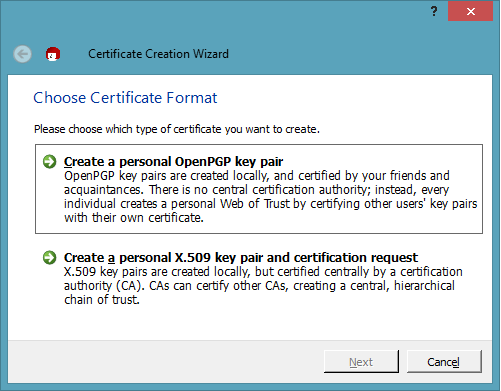
\includegraphics[width=1.2\linewidth]{pics/1.png}}
\caption{Recent Best}
\label{ris:image1}
\end{figure}

Все характеристики не ниже 90. SSL/TLS настроен в соответсвии с лучшими практиками.\\

Из Recent Worst был выбран домен acs-inc.com. Сайт имеет оценку F. Отчет представлен на рисунке 2.

\begin{figure}[!h]	\center{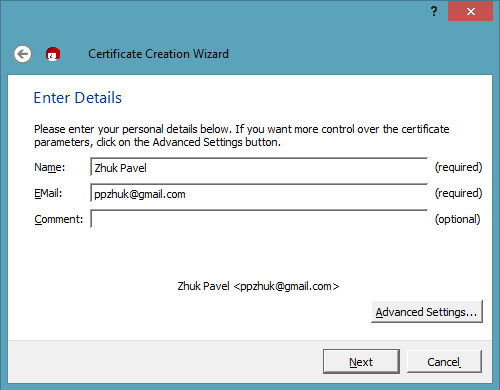
\includegraphics[width=1.2\linewidth]{pics/2.png}}
\caption{Recent Worst}
\label{ris:image2}
\end{figure}

Дополнительно отмечается что сайт подвержен атаке типа DROWN. Это и является причиной присвоенного сайту рейтинга. 

Атака DROWN - это атака, связанная с протоколом TLS, и осуществима в том случае, если осуществляется поддержка небезопасного протокола SSL2.
\subsubsection{Выбрать домен для анализа. Проанализировать}
Для самостоятельного анализа возьмем домен mail.ru.\\

\textbf{Summary}\\
Результаты анализа приведены на рисунке 3. Сайт имеет категорию А+ - максимально возможную оценку. Замечания отсутсвуют. Дополнительно отмечена поддержка HSTS.

\begin{figure}[!h]	\center{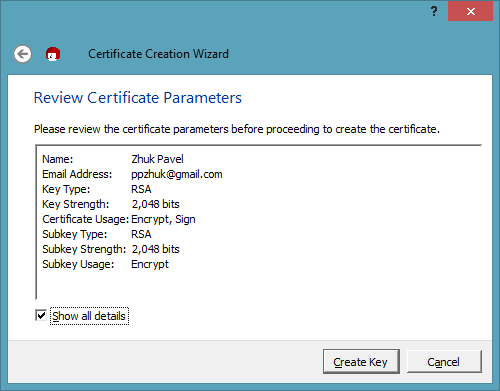
\includegraphics[width=1.2\linewidth]{pics/3.png}}
\caption{Анализ mail.ru}
\label{ris:image3}
\end{figure}

\textbf{Configuration}\\

Расшифруем аббривиатуры из раздела Cobfiguration, представленные ниже.

\begin{verbatim}
TLS_ECDHE_RSA_WITH_AES_256_GCM_SHA384 (0xc030)   ECDH secp256r1 (eq. 3072 bits RSA)   FS	256
TLS_ECDHE_RSA_WITH_AES_128_GCM_SHA256 (0xc02f)   ECDH secp256r1 (eq. 3072 bits RSA)   FS	128
TLS_ECDHE_RSA_WITH_AES_256_CBC_SHA384 (0xc028)   ECDH secp256r1 (eq. 3072 bits RSA)   FS	256
TLS_ECDHE_RSA_WITH_AES_128_CBC_SHA256 (0xc027)   ECDH secp256r1 (eq. 3072 bits RSA)   FS	128
TLS_ECDHE_RSA_WITH_AES_256_CBC_SHA (0xc014)   ECDH secp256r1 (eq. 3072 bits RSA)   FS	256
TLS_ECDHE_RSA_WITH_AES_128_CBC_SHA (0xc013)   ECDH secp256r1 (eq. 3072 bits RSA)   FS	128
TLS_ECDHE_RSA_WITH_3DES_EDE_CBC_SHA (0xc012)   ECDH secp256r1 (eq. 3072 bits RSA)   FS	112
TLS_DHE_RSA_WITH_AES_256_GCM_SHA384 (0x9f)   DH 2048 bits   FS	256
TLS_DHE_RSA_WITH_AES_256_CBC_SHA256 (0x6b)   DH 2048 bits   FS	256
TLS_DHE_RSA_WITH_AES_256_CBC_SHA (0x39)   DH 2048 bits   FS	256
TLS_DHE_RSA_WITH_CAMELLIA_256_CBC_SHA (0x88)   DH 2048 bits   FS	256
TLS_DHE_RSA_WITH_AES_128_GCM_SHA256 (0x9e)   DH 2048 bits   FS	128
TLS_DHE_RSA_WITH_AES_128_CBC_SHA256 (0x67)   DH 2048 bits   FS	128
TLS_DHE_RSA_WITH_AES_128_CBC_SHA (0x33)   DH 2048 bits   FS	128
TLS_DHE_RSA_WITH_SEED_CBC_SHA (0x9a)   DH 2048 bits   FS	128
TLS_DHE_RSA_WITH_CAMELLIA_128_CBC_SHA (0x45)   DH 2048 bits   FS	128
TLS_DHE_RSA_WITH_3DES_EDE_CBC_SHA (0x16)   DH 2048 bits   FS	112
TLS_RSA_WITH_AES_256_GCM_SHA384 (0x9d)	256
TLS_RSA_WITH_AES_256_CBC_SHA256 (0x3d)	256
TLS_RSA_WITH_AES_256_CBC_SHA (0x35)	256
TLS_RSA_WITH_CAMELLIA_256_CBC_SHA (0x84)	256
TLS_RSA_WITH_AES_128_GCM_SHA256 (0x9c)	128
TLS_RSA_WITH_AES_128_CBC_SHA256 (0x3c)	128
TLS_RSA_WITH_AES_128_CBC_SHA (0x2f)	128
TLS_RSA_WITH_CAMELLIA_128_CBC_SHA (0x41)	128
TLS_RSA_WITH_3DES_EDE_CBC_SHA (0xa)	112
TLS_RSA_WITH_SEED_CBC_SHA (0x96)	128
\end{verbatim}

Расшифровки:
\begin{itemize}
\item TLS - протокол защищенной передачи данных;
\item ECDHE / ECDH / DH - алгоритм Диффи-Хэлмана на эллиптических кривых;
\item RSA - алгоритм шифрования с открытым ключем;
\item AES\_128 - алгоритм шифрования с длиной ключа в 128 бит;
\item GCM - режим блочного шифрования;
\item SHA256 - хэш-функция с длиной ключа 256 бит;
\item FS - forward secrecy;
\item CBC - режим блочного шифрования;
\item CAMELLIA - симметричный блочный шифр;
\item 3DES - симметричный блочный шифр;
\item SEED - симметричный блочный шифр;
\end{itemize}

\textbf{Protocol Details}\\
Прокомментируем данный раздел подробнее.

\begin{verbatim}
DROWN (experimental)	No, server keys and hostname not seen elsewhere with SSLv2
BEAST attack	Not mitigated server-side (more info)   TLS 1.0: 0xc014
POODLE (SSLv3)	No, SSL 3 not supported (more info)
POODLE (TLS)	No (more info)
Downgrade attack prevention	Yes, TLS_FALLBACK_SCSV supported (more info)
\end{verbatim}
Сайт не подвержен атакам DROWN, BEAST, POODLE (SSLv3), POODLE (TLS), Downgrade (понижение версии протоколов).

\begin{verbatim}
Secure Renegotiation	Supported
\end{verbatim}
Поддерживается защищенное переподключение.

\begin{verbatim}
Secure Client-Initiated Renegotiation	No
Insecure Client-Initiated Renegotiation	No
\end{verbatim}
Любые виды переподключения по инициативе клиента запрещены.

\begin{verbatim}
SSL/TLS compression	No
RC4	No
\end{verbatim}
Потоковый шифр и сжатие отключены.

\begin{verbatim}
Heartbeat (extension)	Yes
Heartbleed (vulnerability)	No (more info)
\end{verbatim}
Сайт защищен от heartbleed.

\begin{verbatim}
OpenSSL CCS vuln. (CVE-2014-0224)	No (more info)
OpenSSL Padding Oracle vuln.
(CVE-2016-2107)	No (more info)
\end{verbatim}
Отсутсвуют данные уязвимости.

\begin{verbatim}
Forward Secrecy	Yes (with most browsers)   ROBUST (more info)
\end{verbatim}
Имеется поддержка Forward Secrecy для большинства собверменных браузеров.

\begin{verbatim}
ALPN	Yes
NPN	Yes   http/1.1
\end{verbatim}
Поддерживается протокол ALPN (Application-Layer Protocol Negotiation) и его более ранняя версия NPN.


\begin{verbatim}
Strict Transport Security (HSTS)	Yes 
max-age=16070400
HSTS Preloading	Not in: Chrome  Edge  Firefox  IE  Tor 
\end{verbatim}
Имеетмя поддержка HSTS.

\begin{verbatim}
Public Key Pinning (HPKP)	No
Public Key Pinning Report-Only	No
\end{verbatim}
Технология привязки ключей не поддерживается.\\

\textbf{Вывод}\\
 Домен mail.ru имеет наивысшую оценку (А+) по реализации SSL. Сайт защищен от всех тестируемых видов атак. Также поддерживаются: Forward Security для современных браузеров, ALPN, возможность возобновления сессии при помощи механизма кеширования и другое. Можно сделать вывод о хорошей защищенности данного сайта.
 
\section{Вывод}
В ходе данной лабораторной работы были изучены возможности сервиса SSL Labs, анализирующего качество защиты домена.

Были рассмотрены отчеты для сервисов с высокой и низкой оценками. Также был проанализирован домен mail.ru. Был просмотрен отчет по данному домену,  и изучены детали: используемые способы шифрования, защита от уязвимстей и другое. В результате был сделан вывод, что сайт mail.ru является хорошо защищенным.
\end{document}
